
\documentclass[11pt]{article}
\usepackage[T1]{fontenc}
\usepackage{lmodern}
\usepackage[letterpaper,margin=0.80in]{geometry}
\usepackage{amsmath,amssymb,booktabs,graphicx}
\usepackage[hidelinks]{hyperref}
\setlength{\emergencystretch}{2em}
\makeatletter
\setlength{\@fptop}{0pt}
\setlength{\@fpsep}{18pt}
\makeatother
\hypersetup{pdftitle={Spectrally constrained stochastic factorization for low-dose CT}}
\begin{document}
\begin{center}
  \Large\bfseries Spectrally constrained stochastic factorization for low-dose CT
\end{center}

\section{Low-dose CT reconstruction model}
We reconstruct a two-dimensional attenuation image from X-ray measurements
taken at several angles. Attenuation describes how strongly material reduces
the transmitted intensity per unit distance. At one angular position, called
a view, an X-ray source illuminates a line of detector bins. The source-to-bin
rays spread out in a fan. Under the Beer--Lambert model, the negative logarithm
of intensity relative to unobstructed illumination approximates a line integral
of attenuation \cite{detect}.

Treat \(X_{pq}\) as the constant attenuation in pixel \((p,q)\) on a
\(512\times512\) grid. If \(\ell_{ij,pq}\) is the length in millimeters
of ray \(j\) in view \(i\) within that pixel, the calibrated forward map is
\[
  P_i\colon\mathbb R^{512\times512}\longrightarrow\mathbb R^d,\qquad
  [P_i(X)]_j=\sum_{p,q}\ell_{ij,pq}X_{pq},\qquad d=956.
\]
The fixed source and detector geometry determines these weights. ASTRA traces
the rays to apply this map to selected views \cite{astra}.

We write the image as \(X=UV^\top\) with \(U,V\in\mathbb R^{512\times64}\),
restricting its rank to at most \(64\). All views constrain the same factors.
For measured view data \(y_i\in\mathbb R^d\), the unweighted loss is
\[
  f(U,V) = \frac{1}{N}\sum_{i\in\mathcal I_{\rm train}}
    \frac{\|P_i(UV^\top)-y_i\|_2^2}{2d},
  \qquad N=|\mathcal I_{\rm train}|.
\]
The loss is quadratic in the image and nonconvex in the factors. To bound
factor scale, use spectral-norm caps
\(C=\{(U,V):\|U\|_{\rm op}\le R_U,\ \|V\|_{\rm op}\le R_V\}\).
Each radius is twice the operator norm of the corresponding calibrated warm
factor. Nonnegative factors give a nonnegative attenuation image, so define
\(D=\{(U,V):U\ge0,\ V\ge0\}\) entrywise. Write \(g=\iota_D\) for the
function that is zero on \(D\) and infinite elsewhere. Since \(g\) acts
directly on the factors, \(T\) is the identity. With \(x=(U,V)\), the
problem has the SFRAMES form
\[
  \min_{x\in C}\{f(x)+g(Tx)\}.
\]
The component gradients are Lipschitz on the compact region \(C\). Strictly
positive sufficiently small factors lie in the interiors of both \(C\) and
\(D\).

The adjoint \(P_i^\ast\), called backprojection, distributes each detector
residual to the pixels crossed by its ray using the same ray-length weights.
For a uniform minibatch \(B\) of training views, define
\[
  E_B=\frac{1}{|B|d}\sum_{i\in B}P_i^\ast\bigl(P_i(UV^\top)-y_i\bigr),
  \qquad \widehat\nabla f_B(U,V)=(E_BV,E_B^\top U).
\]
This estimator is unbiased conditional on the current factors. One joint
gradient invocation applies one forward projection and one adjoint over
\(B\). An alternating method requests one of the two factor gradients at
its block query point.


\section{Data and evaluation protocol}
The inputs are measured fan-beam sinograms from 2DeteCT \cite{detect}.
A sinogram stacks the detector readings over the angular views of one slice.
We fit the Mode~1 low-dose measurements. The image reference is the published
Mode~2 reconstruction from a separate high-dose acquisition of the same slice.
The two sample mixes label different specimen tubes, with three evaluation
cross sections from each tube.

Each raw Mode~1 sinogram has \(3{,}601\) views and \(1{,}912\) detector cells.
We discard the repeated final view and sum adjacent detector cells. A dark
field measures detector offset and two flat fields measure unobstructed
illumination. After the same detector binning, let \(S_i,D_{\rm dark}\)
and \(F_{\rm flat}\) denote the measurement, dark field and mean flat field.
The processed measurement before detector reversal is
\[
  -\log\!\left(\max\!\left\{
    \frac{S_i-D_{\rm dark}}{F_{\rm flat}-D_{\rm dark}},10^{-6}
  \right\}\right).
\]
We reverse the detector axis to match the DeepInverse convention
\cite{deepinv}. All eight selected acquisitions have zero transmission
clipping counts. Each processed sinogram has \(3{,}600\times956\) entries.

ASTRA 2.5.0 applies the CPU \texttt{line\_fanflat} operator in millimeters
\cite{astra}. The source-to-origin distance is \(431.019989\)~mm, the
origin-to-detector distance is \(97.980499\)~mm and the binned detector
spacing is \(0.1496\)~mm. The square field has width \(116.528143\)~mm and
center \((-0.113797,-0.113797)\)~mm. View \(i\) has angle
\(\pi-2\pi i/3600\). The factors use FP64 arithmetic and the projector
uses FP32. To align the published \(1024\times1024\) reference with the
fitting grid, we flip it vertically, divide by its native voxel width
\(0.113797\)~mm, then average \(2\times2\) pixel blocks.

Views have indices \(0,\ldots,3599\). The training set uses residue zero modulo
ten for \(360\) views and residues zero, three, and six for \(1{,}080\)
views. Both settings reserve residue nine for \(360\) held-out views. The
\(120\) indices divisible by \(30\) calibrate the same warm start for both
training sizes. Calibration views belong to both training sets. Held-out
views are disjoint from training and calibration. Increasing the number of
training views changes the finite sum while preserving the image and factor
dimensions.

The development slices are 04300, 03150.
Table~\ref{tab:sample-slices} lists the evaluation slices. Each slice is
reconstructed separately. The stochastic methods are paired at seed labels
202, 203, 204. Development uses oracle seed label
110. Each oracle generator
uses its seed label plus \(100{,}000\). Calibration uses seed
110 in development and
201 in evaluation. It is fixed within a
slice across methods, oracle seeds, and view counts. Full-batch SFRAMES and PALM
each run once per slice and training size and provide shared references for
the stochastic pairs.

\begin{table}[!htbp]
\centering
\caption{Fresh evaluation slices. All belong to the post-replacement detector regime.}
\label{tab:sample-slices}
\small
\setlength{\tabcolsep}{4pt}
\begin{tabular}{@{}ll@{}}
\toprule
Sample mix & Evaluation slices \\
\midrule
Mix 2 & 03041, 03381, 03611 \\
Mix 3 & 03791, 04131, 04931 \\
\bottomrule
\end{tabular}
\end{table}

\section{Calibration and initialization}
Let \(P_J\) stack the \(120\) calibration views. We divide
\((P_J^\ast y_J)_+\) entrywise by \(P_J^\ast P_J\mathbf1\), floored at
\(10^{-3}\) times its maximum. From a thin SVD of this image, each
rank-\(64\) factor column uses the positive or negative singular-vector
parts with the larger product of norms, with the corresponding singular-value
scaling. We add independent uniform \([0,1)\) entries multiplied by
\(10^{-3}\) times the RMS of each factor. Finally, we fit a scalar
amplitude by least squares on the calibration views, with lower bound
\(10^{-6}\), and multiply both factors by its square root.

Write the resulting factors as \(U_{\rm cal},V_{\rm cal}\).
The spectral radii are
\(R_U=2\|U_{\rm cal}\|_{\rm op}\) and
\(R_V=2\|V_{\rm cal}\|_{\rm op}\).
All expanded evaluation runs start at these common feasible factors in
\(C\cap D\). The earlier LMO initialization outside \(D\) belongs to the
separate pilot ablation. The expanded trajectories therefore begin at
\(d_D=0\), and the first SFRAMES update leaves \(D\).

Starting with a normalized all-ones image, ten power iterations on
\(P_J^\ast P_J\) estimate its largest eigenvalue. Divide this estimate by
\(120d\) to obtain \(\widehat\lambda\). The empirical curvature scales
and smoothing prefactor are
\[
  L_U=\widehat\lambda\|V_{\rm cal}\|_{\rm op}^2,\qquad
  L_V=\widehat\lambda\|U_{\rm cal}\|_{\rm op}^2,\qquad
  \mu_0=1/\max(L_U,L_V).
\]
These scales remain fixed during optimization.

\begin{table}[!htbp]
\centering
\caption{Calibrated spectral caps and empirical curvature scales. Values are rounded for display. Each slice shares these settings across methods, seeds, and training-view counts.}
\label{tab:calibration}
\small
\setlength{\tabcolsep}{4pt}
\begin{tabular}{@{}lrrrrr@{}}
\toprule
Slice & $R_U$ & $R_V$ & $L_U$ & $L_V$ & $\mu_0$ \\
\midrule
04300 & $3.9529$ & $3.9415$ & $0.19332$ & $0.19443$ & $5.1431$ \\
03150 & $3.7934$ & $3.7924$ & $0.17897$ & $0.17906$ & $5.5846$ \\
03041 & $3.7261$ & $3.7247$ & $0.17264$ & $0.17277$ & $5.7881$ \\
03381 & $3.4379$ & $3.435$ & $0.14682$ & $0.14707$ & $6.7994$ \\
03611 & $3.8419$ & $3.8475$ & $0.18421$ & $0.18367$ & $5.4286$ \\
03791 & $3.7472$ & $3.7484$ & $0.17484$ & $0.17472$ & $5.7195$ \\
04131 & $3.7834$ & $3.7811$ & $0.1779$ & $0.17812$ & $5.6141$ \\
04931 & $3.9813$ & $3.9806$ & $0.19718$ & $0.19724$ & $5.07$ \\
\bottomrule
\end{tabular}
\end{table}

\section{Optimizers and rate selection}
For \(k\ge0\), both SFRAMES variants use
\[
  \gamma_k=\gamma_0/(k+1)^{3/4},\qquad
  \rho_k=1/(k+1)^{1/2},\qquad
  \mu_k=\mu_0/(k+1)^{1/4}.
\]
Minibatch SFRAMES draws 64
training views uniformly without replacement at each step, independently across
steps. Its full-batch
counterpart uses every training view and tunes its own \(\gamma_0\). The
momentum starts with the first gradient and subsequently satisfies
\[
  m_k=(1-\rho_k)m_{k-1}+\rho_k\widehat\nabla f_{B_k}(x_k),\qquad k\ge1.
\]
Both add the orthant Moreau gradient after this averaging and update by
\[
  s_k=\operatorname{LMO}_C\!\left(m_k+
       \frac{x_k-\Pi_D(x_k)}{\mu_k}\right),\qquad
  x_{k+1}=(1-\gamma_k)x_k+\gamma_k s_k.
\]
Here \(\Pi_D\) clips negative entries, so the Moreau term is the negative
part of each factor divided by \(\mu_k\) \cite{sframes}.
For a block direction with thin singular
value decomposition \(G=A\operatorname{diag}(\sigma)B^\top\), the exact
oracle is \(-RA_+B_+^\top\), with singular vectors restricted to positive
singular values. Its optimal value is \(-R\|G\|_*\), where the star denotes
the nuclear norm. The FP64 implementation retains singular values exceeding
\(\varepsilon_{\rm mach}\max(\operatorname{shape}G)\sigma_{\max}(G)\)
and returns zero for a zero direction. Discarding small singular values gives
an oracle support-gap bound of \(R\) times their sum. Each SFRAMES update
uses two \(512\times64\) thin SVDs, one for each factor.

SPRING--SARAH updates \(U\), then \(V\) using the new \(U\), with steps
\(a/L_U\) and \(a/L_V\). Each block independently refreshes its estimator
with probability \(1/q\) using all training views. Both blocks begin with
full gradients at their respective query points. Between refreshes, a
\(64\)-view SARAH difference updates each estimator \cite{spring}.
ProxSARAH uses a joint step \(a/(L_U+L_V)\), a \(256\)-view snapshot,
then \(m\) recursive updates with \(64\)-view differences before the next
snapshot. Its relaxation is \(0.8\) \cite{proxsarah}. Each recursive
difference evaluates the same sampled views at its two query points. All
subset samples are uniform without replacement within a batch.
PALM uses every training view per alternating block step with the same
curvature scaling as SPRING--SARAH \cite{palm}. Proximal block steps
project onto the spectral-ball and orthant intersection using a single-set
shortcut when feasible and Dykstra iterations with a numerical certificate otherwise.
The individual projections clip negative entries or clip singular values at
the radius. Dykstra uses a requested distance tolerance
\(10^{-8}/(k+1)^{1.1}\), at most \(2{,}000\) inner iterations,
and certificate checks after the first iteration, every five iterations, and
at the final iteration. The certificate uses a primal--dual gap with a
roundoff allowance. A reported floating-point floor can terminate the
projection before the requested tolerance is attained.
The work count includes both evaluations in each recursive difference and all
views used for refreshes and snapshots.

\begin{table}[!htbp]
\centering
\caption{Development grid and frozen evaluation settings. Pairs list the step multiplier followed by the refresh period for SPRING--SARAH or the inner-loop length for ProxSARAH.}
\small
\setlength{\tabcolsep}{4pt}
\begin{tabular}{@{}lrl@{}}
\toprule
Variant & Candidates & Selected \\
\midrule
Minibatch SFRAMES & 0.05, 0.1, 0.16, 0.25 & 0.1 \\
Full-batch SFRAMES & 0.1, 0.25, 0.5, 0.8 & 0.1 \\
SPRING--SARAH & (0.7, 16), (1.1, 16), (1.6, 16), (1.1, 8), (1.1, 32) & (1.6, 16) \\
ProxSARAH & (0.9, 12), (1.5, 12), (2.3, 12), (1.5, 6), (1.5, 24) & (2.3, 12) \\
PALM & 0.6, 1.1, 1.6, 2.3 & 2.3 \\
\bottomrule
\end{tabular}
\end{table}

We select each setting by the smallest median ratio of repaired training loss
to initial loss across both development slices and both training sizes. The
ratio uses the last iterate within \(8{,}640\)
forward and adjoint views in each direction. This gives
\(88\) development runs across two slices, two training sizes and
\(22\) candidate settings. Held-out loss and reference-image error are
reporting metrics.
The selected rate lies at the upper grid edge for SPRING--SARAH, ProxSARAH, PALM. The selected rate lies at the lower grid edge for Full-batch SFRAMES. The comparison reflects the settings covered by these grids.


\section{Evaluation results}
132 of 132 evaluation runs completed. The comparison
uses the last saved iterate with at most \(17{,}280\) forward views and
\(17{,}280\) adjoint views. A run stops after the first complete update that
reaches the work budget. When an update crosses the budget, the previous
iterate supplies the within-budget comparison. The tables use saved probes
without interpolation.

An iteration completes one update of both factors. A gradient call applies
one forward operator and one adjoint to the requested batch and returns either
a joint gradient or one block gradient. Both evaluations in each SARAH
difference and all refresh and snapshot views contribute to the work count.
Gradient-call counts therefore describe the implementation, while the two
view counts measure how much projection data the calls process.

Raw loss uses the actual factors. Repaired loss, held-out loss and reference
error use the image formed after taking each factor's positive part and
scaling it down if its operator norm exceeds its cap. Spectral violation is
\(d_C=\max\{(\|U\|_{\rm op}-R_U)_+,
(\|V\|_{\rm op}-R_V)_+\}\). Distance to \(D\) is
\(d_D=(\|\min(U,0)\|_F^2+\|\min(V,0)\|_F^2)^{1/2}\).
Reference error is the Frobenius error relative to the aligned Mode~2 image,
divided by that image's Frobenius norm.

For absolute metrics we take the median over seeds within each slice and then
the median across slices at each training size. Percent differences first
compare paired runs using the comparator in the denominator and then apply
the same aggregation. Each training size has \(18\) paired seed cases from
six slices. Full-batch SFRAMES and PALM provide shared deterministic
references. These summaries are descriptive because the three slices from
each sample mix share a sample tube.

\begin{table}[!htbp]
\centering
\caption{Work at the projection budget of \(17{,}280\) views per direction. Values are medians across slice medians. The last saved iterate can fall below the cap when the next complete update would exceed it.}
\label{tab:work}
\small
\setlength{\tabcolsep}{4pt}
\begin{tabular}{@{}llrrrr@{}}
\toprule
$N$ & Variant & Iterations & Gradient calls & Forward views & Adjoint views \\
\midrule
360 & Minibatch SFRAMES & $270$ & $270$ & $17280$ & $17280$ \\
360 & Full-batch SFRAMES & $48$ & $48$ & $17280$ & $17280$ \\
360 & SPRING--SARAH & $60$ & $233$ & $17144$ & $17144$ \\
360 & ProxSARAH & $125$ & $240$ & $17280$ & $17280$ \\
360 & PALM & $24$ & $48$ & $17280$ & $17280$ \\
1{,}080 & Minibatch SFRAMES & $270$ & $270$ & $17280$ & $17280$ \\
1{,}080 & Full-batch SFRAMES & $16$ & $16$ & $17280$ & $17280$ \\
1{,}080 & SPRING--SARAH & $47$ & $183$ & $16792$ & $16792$ \\
1{,}080 & ProxSARAH & $125$ & $240$ & $17280$ & $17280$ \\
1{,}080 & PALM & $8$ & $16$ & $17280$ & $17280$ \\
\bottomrule
\end{tabular}
\end{table}

\begin{table}[!htbp]
\centering
\caption{Losses, image error and feasibility at the saved within-budget iterates in Table~\ref{tab:work}. All losses use the same detector and view normalization. Values are medians across slice medians.}
\label{tab:metrics}
\small
\setlength{\tabcolsep}{4pt}
\begin{tabular}{@{}llrrrrrr@{}}
\toprule
$N$ & Variant & Raw & Repaired & Held-out & Ref. error & $d_C$ & $d_D$ \\
\midrule
360 & Minibatch SFRAMES & $0.01219$ & $0.0122$ & $0.01238$ & $0.3636$ & $0$ & $0.0104$ \\
360 & Full-batch SFRAMES & $0.0174$ & $0.01746$ & $0.0175$ & $0.4983$ & $0$ & $0.0304$ \\
360 & SPRING--SARAH & $0.01613$ & $0.01613$ & $0.01615$ & $0.4904$ & $0$ & $0$ \\
360 & ProxSARAH & $0.01543$ & $0.01543$ & $0.01547$ & $0.4751$ & $0$ & $0$ \\
360 & PALM & $0.01909$ & $0.01909$ & $0.01909$ & $0.5397$ & $0$ & $0$ \\
1{,}080 & Minibatch SFRAMES & $0.01225$ & $0.01226$ & $0.01235$ & $0.3572$ & $0$ & $0.0102$ \\
1{,}080 & Full-batch SFRAMES & $0.02292$ & $0.02304$ & $0.02299$ & $0.6154$ & $0$ & $0.0661$ \\
1{,}080 & SPRING--SARAH & $0.01735$ & $0.01735$ & $0.01734$ & $0.5116$ & $0$ & $0$ \\
1{,}080 & ProxSARAH & $0.01543$ & $0.01543$ & $0.01543$ & $0.4737$ & $0$ & $0$ \\
1{,}080 & PALM & $0.02362$ & $0.02362$ & $0.02358$ & $0.6165$ & $0$ & $0$ \\
\bottomrule
\end{tabular}
\end{table}

\clearpage
\begin{table}[!htbp]
\centering
\caption{Median paired percent differences for minibatch SFRAMES at \(17{,}280\) views per direction. Negative values favor minibatch SFRAMES. Slices won counts slices with lower median paired repaired loss.}
\label{tab:paired}
\small
\setlength{\tabcolsep}{4pt}
\begin{tabular}{@{}llrrrr@{}}
\toprule
$N$ & Comparator & Pairs & Repaired & Held-out & Slices won \\
\midrule
360 & Full-batch SFRAMES & 18 & $-30.84\%$ & $-29.65\%$ & 6/6 \\
360 & SPRING--SARAH & 18 & $-24.55\%$ & $-23.55\%$ & 6/6 \\
360 & ProxSARAH & 18 & $-21.48\%$ & $-20.52\%$ & 6/6 \\
360 & PALM & 18 & $-36.63\%$ & $-35.62\%$ & 6/6 \\
1{,}080 & Full-batch SFRAMES & 18 & $-48.70\%$ & $-48.37\%$ & 6/6 \\
1{,}080 & SPRING--SARAH & 18 & $-29.39\%$ & $-28.93\%$ & 6/6 \\
1{,}080 & ProxSARAH & 18 & $-21.07\%$ & $-20.72\%$ & 6/6 \\
1{,}080 & PALM & 18 & $-51.31\%$ & $-50.99\%$ & 6/6 \\
\bottomrule
\end{tabular}
\end{table}

At the common work cap, minibatch SFRAMES completes \(270\) updates at both
training sizes. Full-batch SFRAMES completes \(48\) updates with \(360\)
training views and \(16\) with \(1{,}080\) views. The median paired reduction
in repaired training loss relative to full-batch SFRAMES is
\(30.8\%\) with \(360\) training views and \(48.7\%\) with \(1{,}080\) training views.
Minibatch SFRAMES has lower median paired repaired loss than each comparator
on all six evaluation slices at both training sizes. Its held-out loss also
improves relative to every comparator in the overall slice summaries.
Figure~\ref{fig:paired-effects} shows the individual slice effects so that
the variability across slices remains visible.

Figures~\ref{fig:training-trajectories} and~\ref{fig:quality-trajectories}
show the saved loss and feasibility trajectories. These expanded runs use
the shared feasible warm start described above. Both SFRAMES variants leave
\(D\) after the first update and subsequently reduce their orthant distance.
Their loss after feasibility repair remains close to their raw loss at the
work cap. Every saved evaluation probe has zero spectral violation, and the
projection baselines retain nonnegative factors. At every evaluation baseline
projection, clipping to the orthant already satisfies the spectral cap, so
the single-set shortcut applies. The separately
tuned rates and the boundary selections in the development grid limit the
comparison to these practical settings.


\clearpage
\section{Optimization trajectories}
Figures~\ref{fig:training-trajectories} and~\ref{fig:quality-trajectories}
show all five methods at both training-view counts. For display, each saved
seed trajectory is linearly interpolated between diagnostic probes on a common
work grid. We take the pointwise median over seeds within each slice, then the
median across the six slices. Full-batch SFRAMES and PALM contribute one run
per slice and training size. Shading shows the middle \(50\%\) of slice
medians for the two SFRAMES variants. These are descriptive trajectories,
with no extrapolation beyond recorded work. Numerical tables use actual
saved within-budget iterates, so a displayed interpolated endpoint can differ
slightly from a table entry.

Probes were scheduled every \(4{,}320\) forward views in evaluation and
every \(2{,}160\) in development, with extra probes at the first update and
around budget crossings. The spacing limits what can be inferred about
behavior between probes. Forward and adjoint view counts agree at every
saved probe.

\begin{figure}[!htbp]
  \centering
  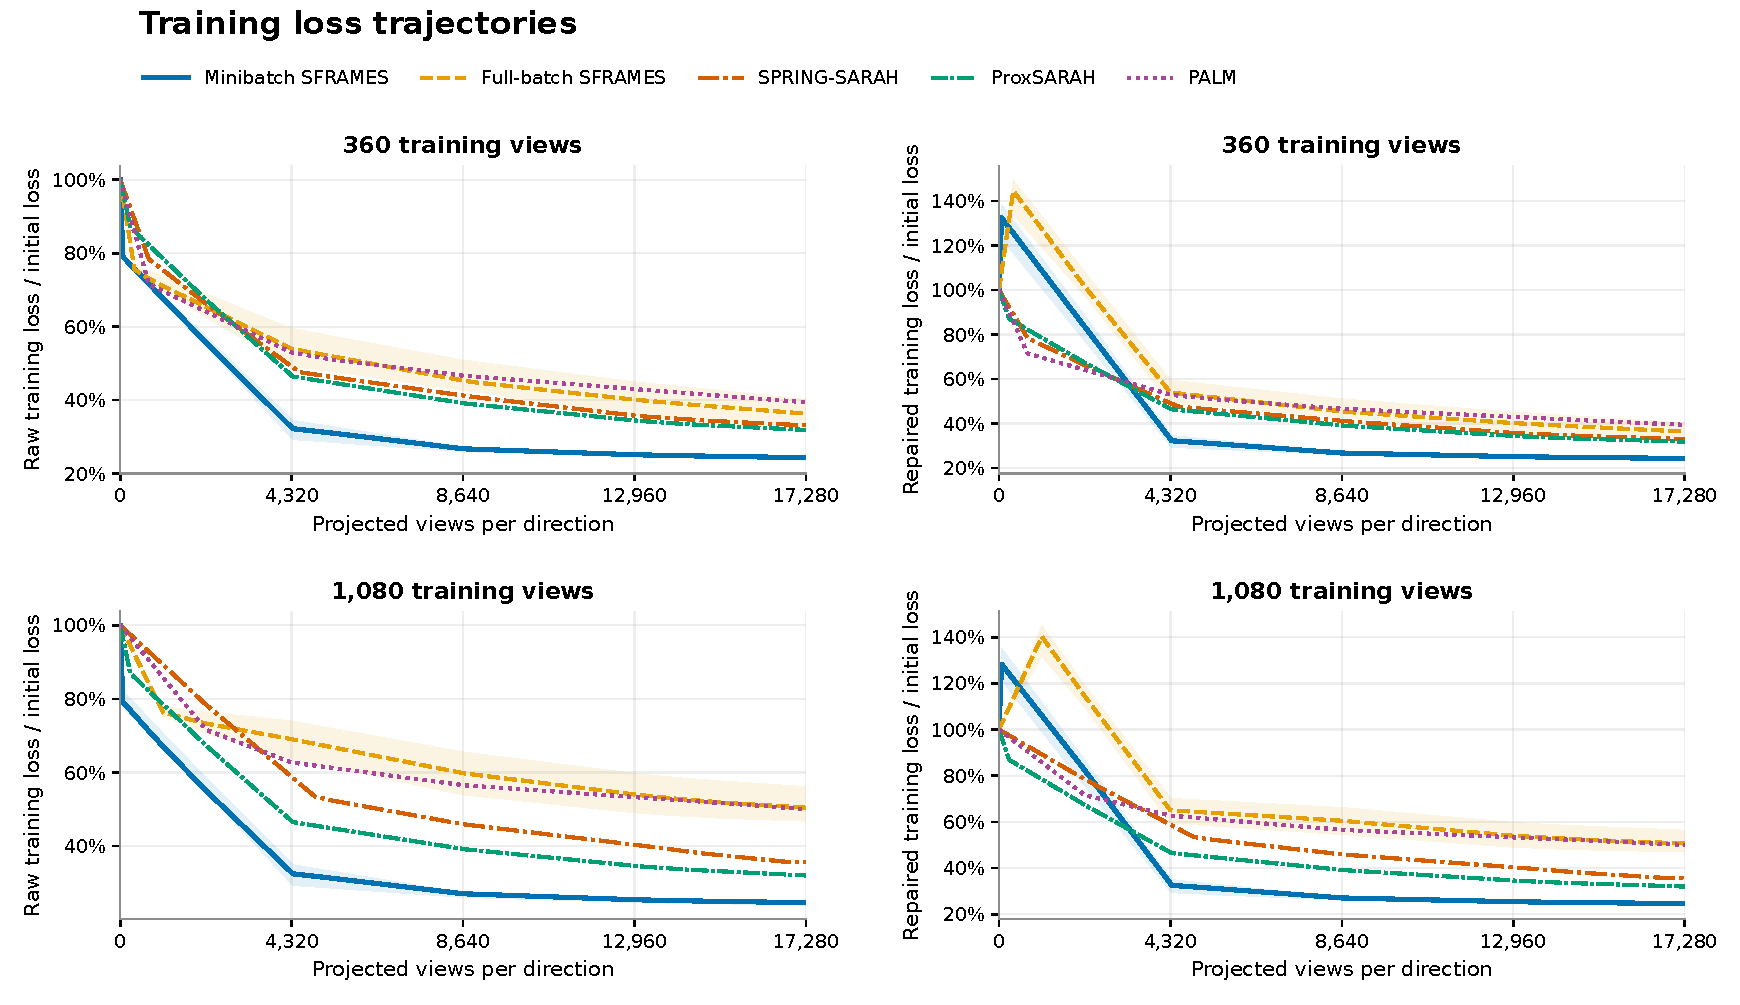
\includegraphics[width=\linewidth]{trajectory_training.pdf}
  \caption{Raw and repaired training loss versus processed views in each
  projection direction. Each loss is divided by its own slice and training
  split's common initial loss before aggregation. Rows compare \(360\) and
  \(1{,}080\) training views.}
  \label{fig:training-trajectories}
\end{figure}
\clearpage
\begin{figure}[!htbp]
  \centering
  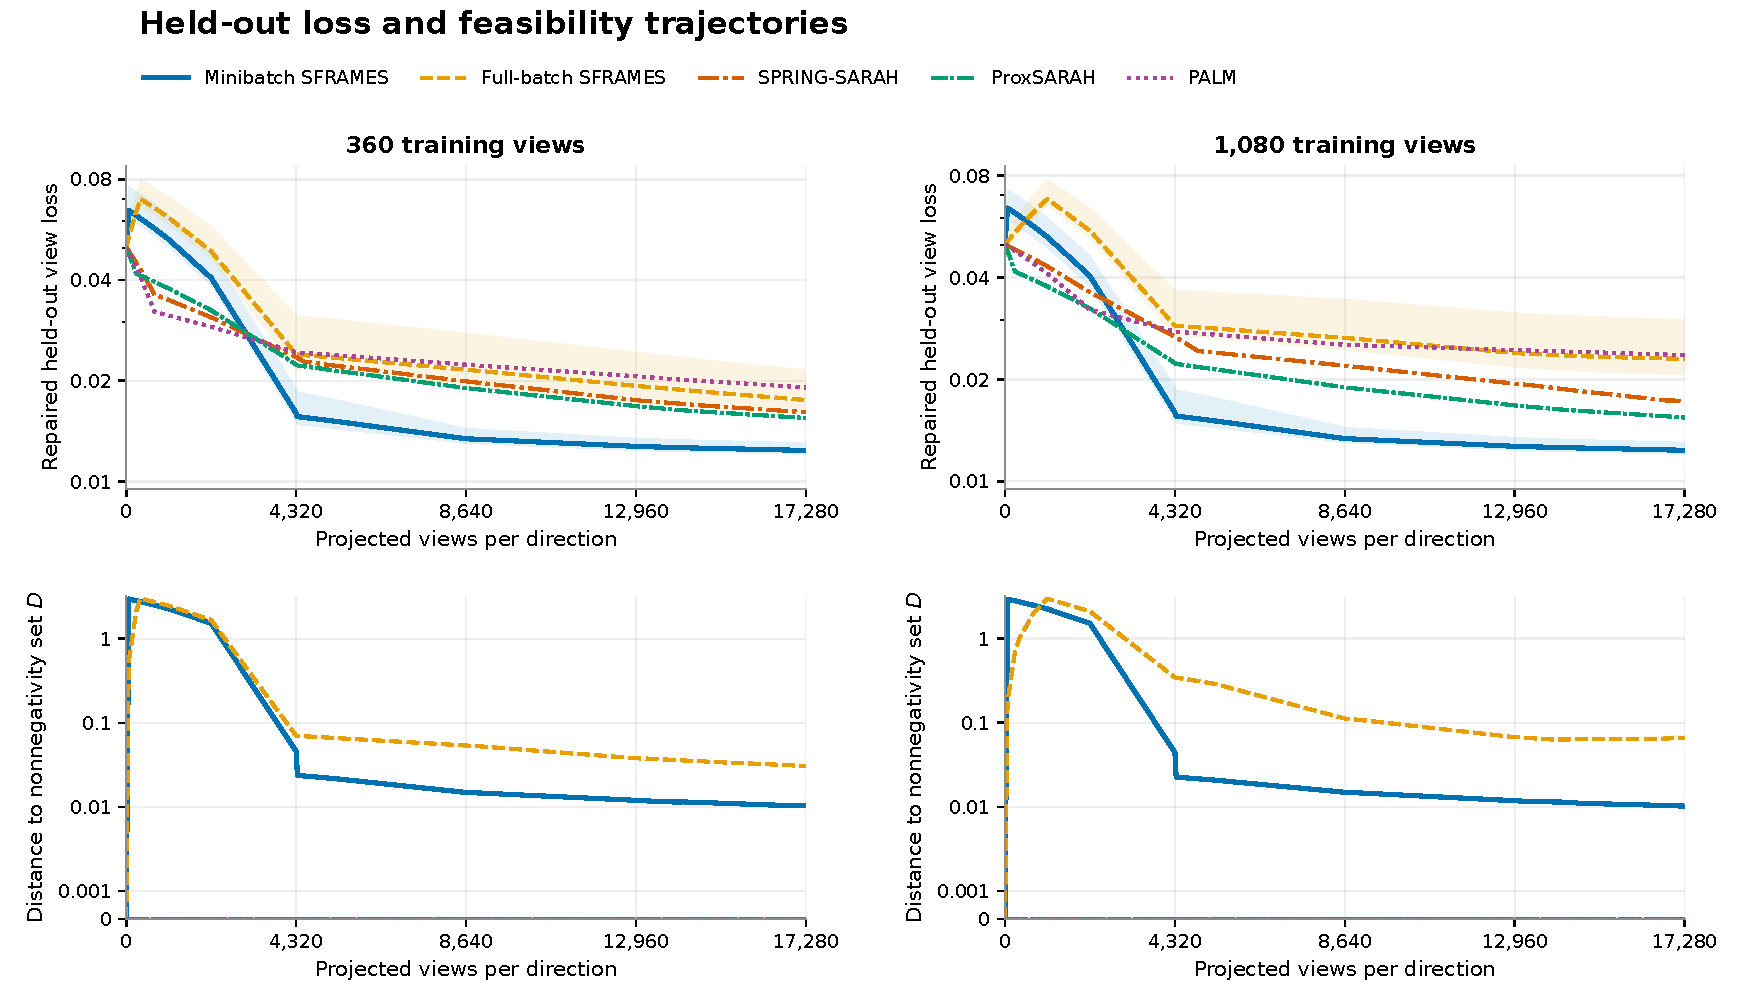
\includegraphics[width=\linewidth]{trajectory_quality.pdf}
  \caption{Held-out loss after factor repair and distance of the raw factors
  to the nonnegative orthant \(D\), versus projection work. The feasibility
  axis uses a symmetric logarithmic scale with a linear region around zero.
  The shared warm start has zero distance to \(D\). SFRAMES leaves \(D\)
  after its first update. The three projection baselines coincide at zero
  distance throughout.}
  \label{fig:quality-trajectories}
\end{figure}
\clearpage
\begin{figure}[!htbp]
  \centering
  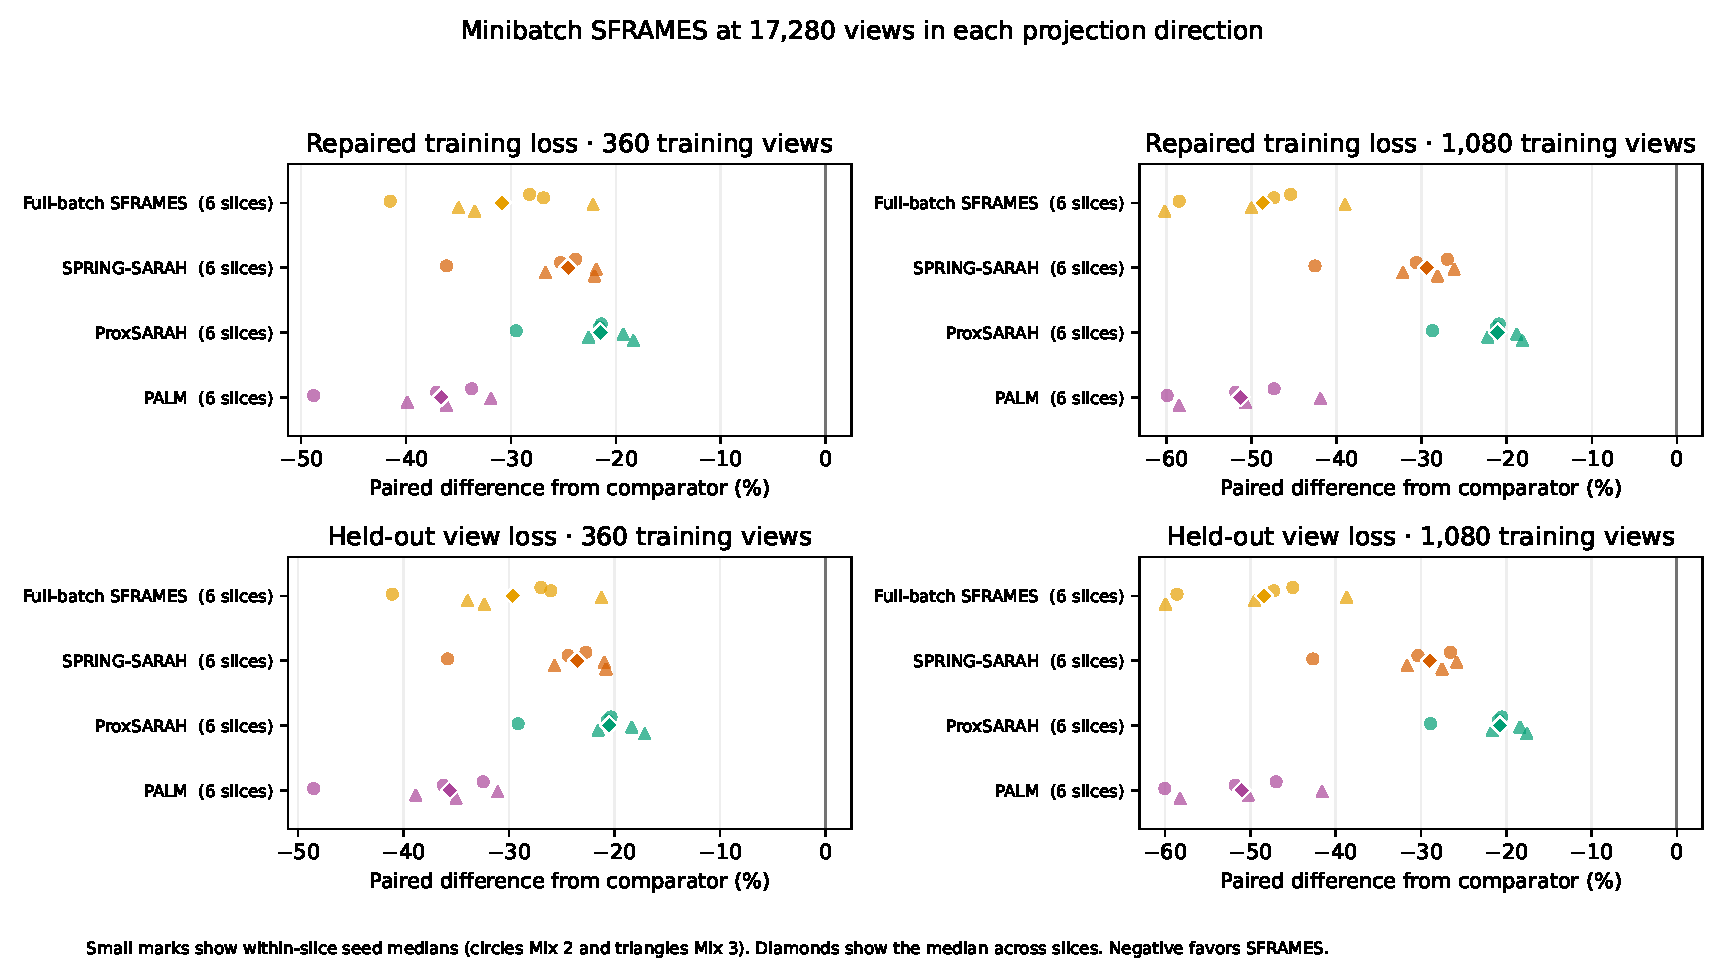
\includegraphics[width=\linewidth]{comparison.pdf}
  \caption{Paired effects for minibatch SFRAMES at the saved within-budget
  iterates. Small marks give the median paired effect over seeds for each
  slice. Circles and triangles distinguish the two sample mixes, and diamonds
  give the median across slices. Negative values favor minibatch SFRAMES.}
  \label{fig:paired-effects}
\end{figure}
\clearpage
\section{Reproduction and scope}
The expanded campaign contains \(88\) development runs and \(132\) fresh
evaluation runs. Per-run configurations and original source, data and
calibration hashes are stored under \texttt{runs/}. The files
\texttt{manifest.json}, \texttt{selection.json} and
\texttt{calibration.json} record the design, frozen rate choices and
calibration checksums. Data sidecars \texttt{data/slice*.json} record the
Zenodo sources, preprocessing conventions and original TIFF checksums.
\texttt{reports/summary.json} records work-based endpoint and paired
summaries. \texttt{analyze.py}, \texttt{plot\_trajectories.py} and
\texttt{report\_latex.py} regenerate the analysis, figures and this document
from saved results.

The comparisons measure optimization progress under the recorded operator
work budget. Concurrent execution on the host does not provide a controlled
timing benchmark. This report uses iterations, gradient-oracle calls and
projection work to characterize the completed runs. The problem size, rank,
initialization, smoothing schedule and projection settings are fixed in this
campaign. Training-view count, stochastic seed and the development rate and
refresh grids supply the reported variations.

\begin{thebibliography}{9}
\bibitem{sframes}
\emph{Improved convergence and stochastic estimation for the Frank--Wolfe
with Moreau Envelope Smoothing (FraMES) algorithm}. Local manuscript,
27 September 2026. Corollary~2.10 and Proposition~2.11.
\bibitem{detect}
M.~B.~Kiss et al.
\emph{2DeteCT: A large 2D expandable, trainable, experimental Computed Tomography
dataset for machine learning}. Scientific Data 10, article 576, 2023.
\href{https://doi.org/10.1038/s41597-023-02484-6}{DOI}.
\bibitem{deepinv}
DeepInverse.
\href{https://deepinv.org/auto_examples/external-libraries/demo_astra_2detect.html}
{Reconstruct real CT sinograms with the 2DeteCT benchmark}.
\bibitem{astra}
ASTRA Toolbox. \href{https://astra-toolbox.com/docs/proj2d.html#fan-beam}{2D Projectors}.
\bibitem{spring}
D.~Driggs, J.~Tang, J.~Liang, M.~E.~Davies, and C.-B.~Sch\"onlieb.
\emph{A Stochastic Proximal Alternating Method for Nonsmooth and Nonconvex Optimization}.
SIAM Journal on Imaging Sciences 14(4), 1932--1970, 2021.
\href{https://doi.org/10.1137/20M1387213}{DOI}.
\bibitem{proxsarah}
N.~H.~Pham, L.~M.~Nguyen, D.~T.~Phan, and Q.~Tran-Dinh.
\emph{ProxSARAH: An Efficient Algorithmic Framework for Stochastic Composite Nonconvex Optimization}.
Journal of Machine Learning Research 21(110), 1--48, 2020.
\href{https://www.jmlr.org/papers/v21/19-248.html}{Article}.
\bibitem{palm}
J.~Bolte, S.~Sabach, and M.~Teboulle.
\emph{Proximal alternating linearized minimization for nonconvex and nonsmooth problems}.
Mathematical Programming 146, 459--494, 2014.
\href{https://doi.org/10.1007/s10107-013-0701-9}{DOI}.
\end{thebibliography}
\end{document}
